\documentclass[unknownkeysallowed]{beamer}
\mode<presentation>
{
%  \usetheme{AnnArbor}
%  \usetheme{Dresden}
%  \usetheme{Montpellier}
%  \usetheme{Antibes}
%  \usetheme{Frankfurt}
%  \usetheme{PaloAlto}
%  \usetheme{Bergen}
%  \usetheme{Boadilla}
%  \usetheme{Goettingen}
%  \usetheme{Pittsburgh}	%!!
%  \usetheme{Berkeley}
%  \usetheme{Hannover}
%  \usetheme{Rochester}		%!!!
%  \usetheme{Berlin}
%  \usetheme{Ilmenau}
%  \usetheme{Singapore}
  \usetheme{Boadilla}		%viel platz
%  \usetheme{JuanLesPins}
%  \usetheme{Szeged}		%!
%  \usetheme{boxes}
%  \usetheme{Luebeck}
%  \usetheme{Warsaw}
%  \usetheme{Copenhagen}
%  \usetheme{Madrid}
%  \usetheme{Darmstadt}
%  \usetheme{Malmoe}
%  \usetheme{default}
%  \usetheme{JuanLesPins}

%  \usetheme{Marburg}


%\usefonttheme{professionalfonts}
%	default | professionalfonts | serif |
%	structurebold | structureitalicserif |
%	structuresmallcapsserif
%\useinnertheme{rounded}
%	circles | default | inmargin |
%	rectangles | rounded

%  \setbeamercovered{transparent}
  % oder auch nicht
\usecolortheme{rose}


\definecolor{uaf yellow}{cmyk}{0,0.16,1,0} % official UAF yellow
\definecolor{light yellow}{cmyk}{0.01,0,0.16,0}
\definecolor{uaf blue}{cmyk}{1,0.66,0,0.02} % official UAF blue
\definecolor{light blue}{cmyk}{0.22,0.11,0,0}
\definecolor{arsc blue}{HTML}{005496}
\definecolor{arsc red}{HTML}{a20a42}
\definecolor{arsc green}{HTML}{009a82}
\definecolor{light gray}{HTML}{777777}

  %navigation aus, klaut nur platz
  \setbeamertemplate{navigation symbols}{}
% Reset title background to default
%\setbeamertemplate{title page}[default]
\setbeamercolor{title}{bg=}
\setbeamercolor{frametitle}{bg=uaf blue, fg=white}
\setbeamercolor{institute}{fg=white}
\setbeamercolor{date}{fg=white}
\setbeamercolor{block}{bg=}
%\setbeamercolor{title}{fg=black}

% Reset block background to default
%\setbeamertemplate{blocks}[default]
%\setbeamercolor{block title}{bg=}
%\setbeamercolor{block body}{bg=}

\beamertemplatenavigationsymbolsempty  
\setbeamertemplate{blocks}[rounded][shadows=false]

\useinnertheme{circles}

}
\usepackage[latin1]{inputenc}
\usepackage{latexsym}
\usepackage{amsfonts}
%\usepackage{natbib}
\usepackage{fancyhdr}
\usepackage{graphicx}
%\usepackage{subfigure}
% oder was auch immer
\usepackage{grffile}
\usepackage{pgf}
\usepackage{tikz}

\usepackage{listings}

\usepackage{times}
\usepackage[T1]{fontenc}
%\usepackage{appendixnumber}
% Oder was auch immer. Zu beachten ist, das Font und Encoding passen
% m�ssen. Falls T1 nicht funktioniert, kann man versuchen, die Zeile
% mit fontenc zu l�schen.

\hypersetup{
    bookmarks=true,         % show bookmarks bar?
    unicode=false,          % non-Latin characters in Acrobat's bookmarks
    pdftoolbar=true,        % show Acrobat's toolbar?
    pdfmenubar=true,        % show Acrobat's menu?
    pdffitwindow=false,     % window fit to page when opened
    pdfstartview={FitH},    % fits the width of the page to the window
    pdftitle={My title},    % title
    pdfauthor={Author},     % author
    pdfsubject={Subject},   % subject of the document
    pdfcreator={Creator},   % creator of the document
    pdfproducer={Producer}, % producer of the document
    pdfkeywords={keyword1} {key2} {key3}, % list of keywords
    pdfnewwindow=true,      % links in new window
    colorlinks=false,       % false: boxed links; true: colored links
    linkcolor=red,          % color of internal links
    citecolor=green,        % color of links to bibliography
    filecolor=magenta,      % color of file links
    urlcolor=cyan           % color of external links
}

\title[PAG]% (optional, nur bei langen Titeln n�tig)
{GEOS 436 / 636\\
Programming and Automation for Geoscientists\\[20pt]
-- Week 10: Unix -- Scrubbing Data --
}

\author[Grapenthin]% (optional, nur bei vielen Autoren)
{Ronni Grapenthin\\
rgrapenthin@alaska.edu\\
Elvey 413B\\
x7682}
% - Namen m�ssen in derselben Reihenfolge wie im Papier erscheinen.
% - Der \inst{?} Befehl sollte nur verwendet werden, wenn die Autoren
%   unterschiedlichen Instituten angeh�ren.

\institute[UAF] % (optional, aber oft n�tig)
{}
% - Der \inst{?} Befehl sollte nur verwendet werden, wenn die Autoren
%   unterschiedlichen Instituten angeh�ren.
% - Keep it simple, niemand interessiert sich f�r die genau Adresse.

% - Namen m�ssen in derselben Reihenfolge wie im Papier erscheinen.
% - Der \inst{?} Befehl sollte nur verwendet werden, wenn die Autoren
%   unterschiedlichen Instituten angeh�ren.

% - Der \inst{?} Befehl sollte nur verwendet werden, wenn die Autoren
%   unterschiedlichen Instituten angeh�ren.
% - Keep it simple, niemand interessiert sich f�r die genau Adresse.

\date[]{}

% - Volle oder abgek�rzter Name sind m�glich.
% - Dieser Eintrag ist nicht f�r das Publikum gedacht (das wei�
%   n�mlich, bei welcher Konferenz es ist), sondern f�r Leute, die diese
%   Folien sp�ter lesen.

%\AtBeginSection[]
%{
%  \begin{frame}<beamer>
%    \frametitle{Outline}
%    \tableofcontents[currentsection,currentsubsection]
%  \end{frame}
%}

% Falls Aufz�hlungen immer schrittweise gezeigt werden sollen, kann
% folgendes Kommando benutzt werden:

%\beamerdefaultoverlayspecification{<+->}

%%switch on to have only frame numbers
\setbeamertemplate{footline}[frame number]

\defbeamertemplate*{title page}{customized}[1][]
{
		\begin{tikzpicture}
			\node[text width=\textwidth,
				fill=gray!70, 
				fill opacity=0.75,
				text opacity=1,
				rounded corners = 10pt,
				inner sep=2pt]{
				\begin{center}	
			  \usebeamerfont{title}{\bf \usebeamercolor[fg]{title} \inserttitle}
			  \par
			  \usebeamerfont{subtitle}\insertsubtitle\par
			  \bigskip
			  \usebeamerfont{author}\insertauthor\par
			  \bigskip
			  \usebeamerfont{institute}\insertinstitute\par
			  \bigskip
			  \usebeamerfont{date}\insertdate\par
			  \end{center}
			  };
	\end{tikzpicture}		  
%	\vspace{0.4cm}\usebeamercolor[fg]{titlegraphic}\inserttitlegraphic 
%	\begin{flushright}
%	\vspace{-1.25cm}\includegraphics[width=2cm]{../moore_logo_transp.png}\vspace{5cm}
%	\end{flushright}
}

\begin{document}

\lstset{numbers=left, numberstyle=\tiny, stepnumber=2, basicstyle=\ttfamily, numbersep=5pt, xleftmargin=10pt}

\setbeamertemplate{background}{\includegraphics[width=\paperwidth]{/home/roon/Pictures/rooftop_initial.jpg}}

	\begin{frame}
	\begin{center}
		\titlepage
	\end{center}
	\end{frame}

\setbeamertemplate{background}{}

\begin{frame}
\frametitle{}
%	\vspace{2cm}
	\begin{center}
	Are there simple ways to filter, reformat, merge data on the command line?
	\end{center}
%	\vspace{4cm}
%	{\tiny {\color{gray}$^{*}$hint: YES!!!!}}
\end{frame}

\begin{frame}
	\frametitle{Common Operations on Plain Text}
	\begin{itemize}
		\item Filtering lines or fields
		\item Replacing / deleting values
		\item Merging data
	\end{itemize}
	These operations require generic ways to find text patterns of interest: {\bf Regular Expressions}
\end{frame}

\begin{frame}
	\frametitle{Regular Expressions}
	\begin{itemize}
		\item Set of characters that specify a generic pattern
		\item Example: Format of a simple URL is \emph{www-dot-bunchOfCharactersNumbers-dot-someTopLevelDomain}
		\item Regular Expressions help formalize that
		\item Allow to search and substitute text on the command line easy
		\item Are accepted by many Unix commands, incl. grep, sed, awk, \dots (syntax may vary slightly)
	\end{itemize}
\end{frame}

\begin{frame}
	\frametitle{Simple Regular Expression Symbols}
	(surround regular expressions with single quotes to prevent interpretation by the shell)
	\begin{itemize}
		\item {\tt .} (single period): matches any single character (wildcard)
		\item {\tt B}: matches uppercase `B' (as an example for any letter)
		\item {\tt b}: matches uppercase `b' (as an example for any letter)
		\item {\tt *}: match {\bf zero or more} of the previous pattern
		\item {\tt ?}: match {\bf zero or one} of the previous pattern
		\item {\tt +}: match {\bf one or more} of the previous pattern
		\item {\tt \{ \}}: match {\bf number of occurrences} of the previous pattern
	\end{itemize}
\end{frame}

\begin{frame}
	\frametitle{Simple Regular Expression Symbols}

	\begin{itemize}
		\item {\tt \textasciicircum }: search for pattern at beginning of string (line)
		\item {\tt \$}: end of the string (line)
		\item {\tt \textbackslash}: escape special character
		\item {\tt [ ]}: match range of characters inside brackets
		\item {\tt [\textasciicircum ~]}: DO NOT match range of characters inside brackets
	\end{itemize}

	Non-printable characters:
	\begin{itemize}
		\item {\tt {\textbackslash}t} -- tabulator character
		\item {\tt {\textbackslash}r} -- carriage return
		\item {\tt {\textbackslash}n} -- new line
		\item {\tt {\textbackslash}s} -- white space
	\end{itemize}

	Examples of uses of regular expressions in applications of the unix commandline tools below.
\end{frame}


\begin{frame}
	\frametitle{Powerful Commandline Tools}
	\begin{itemize}
		\item {\tt tr}: translate or delete characters
		\item {\tt grep}: print lines that match patterns
		\item {\tt sed}:  stream editor for filtering and transforming text
		\item {\tt awk}: pattern scanning and text processing language
		\item usually piped into each other in various combinations
	\end{itemize}
\end{frame}

\begin{frame}
	\frametitle{{\tt tr}}
	\begin{itemize}
		\item {\tt tr} is a character-based translator ({\tt sed} is word based)
		\item Common uses: change uppercase to lowercase text, delete specific characters
	\end{itemize}

	\begin{center}
	{\tt tr OPTIONS SET1 [SET2]}
	\end{center}
	\begin{itemize}
		\item translate characters given in {\tt SET1} to those in {\tt SET2}
		\item {\tt -d}: delete characters given in {\tt SET1} (SET2 not needed)
	\end{itemize}

\end{frame}

\begin{frame}
	\frametitle{{\tt tr} Example}
	\begin{center}
		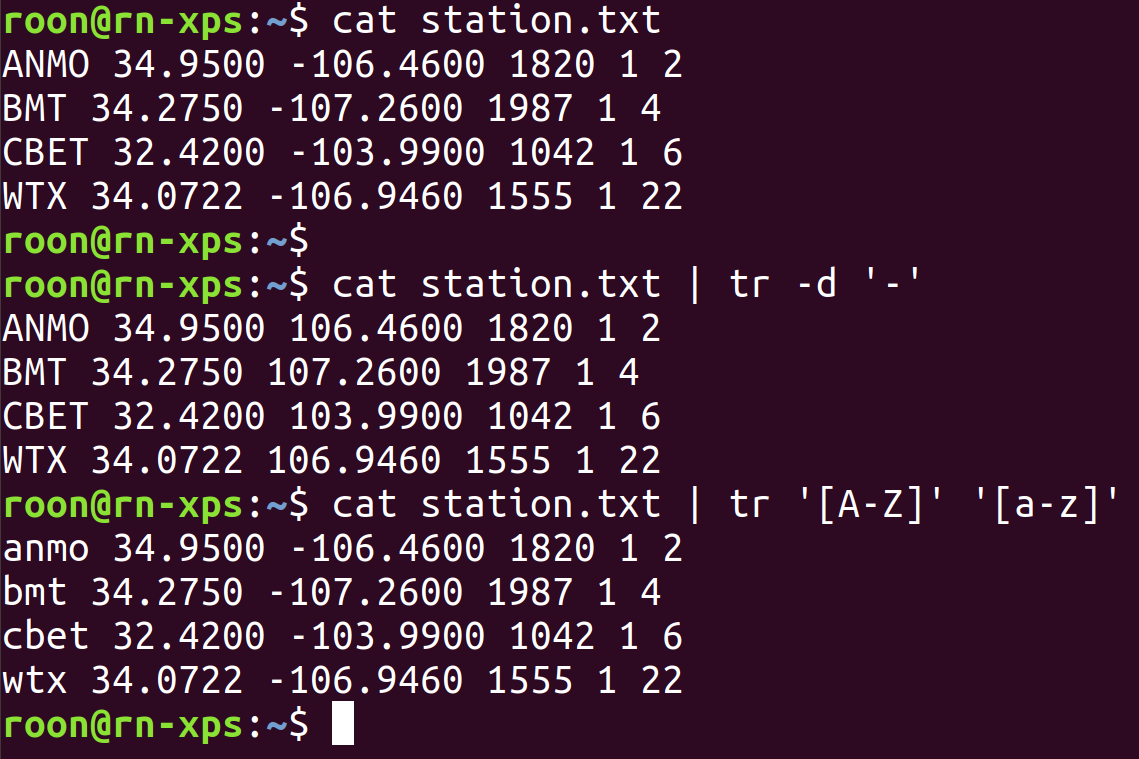
\includegraphics[width=.8\textwidth]{../figures/tr_example.png}	
	\end{center}
\end{frame}

\begin{frame}
	\frametitle{{\tt grep}}
	\begin{itemize}
		\item match lines from input based on search pattern
		\item input can be stdin, one or multiple files!
		\item different versions used to exist, all captured by various options of {\tt grep}
	\end{itemize}

	\begin{center}
	{\tt grep pattern in\_file}
	\end{center}
	\begin{itemize}
		\item All lines in {\tt in\_file} that contain {\tt pattern} are printed
		\item {\tt  pattern} can be a simple string or regular expression ({\tt -E} provides extended implementation)
		\item {\tt grep -v} inverts the pattern and returns only lines that DO NOT match
	\end{itemize}

\end{frame}

\begin{frame}
	\frametitle{{\tt grep} Example}
	\begin{center}
		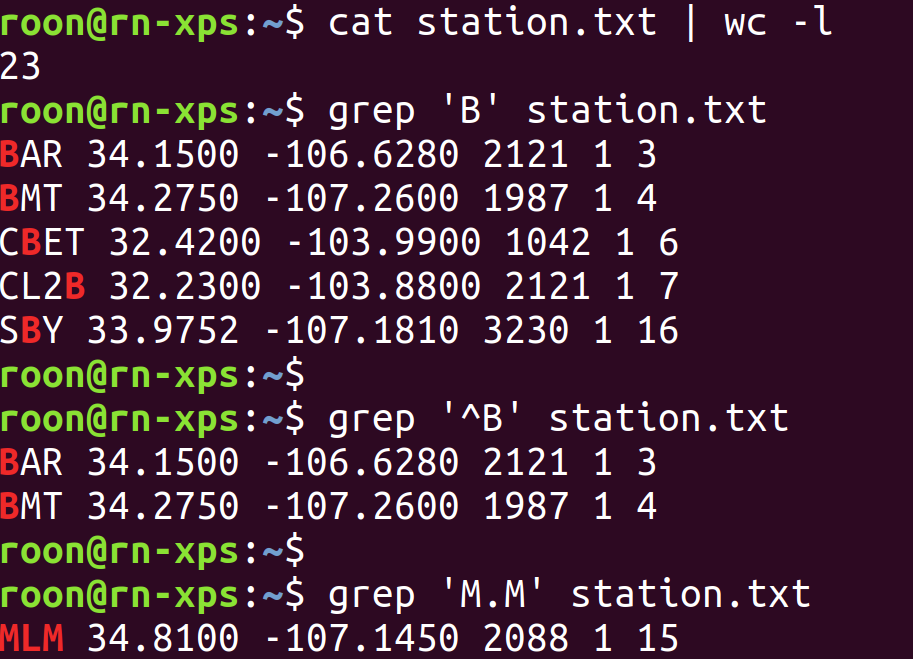
\includegraphics[width=.8\textwidth]{../figures/grep_examples.png}	
	\end{center}
\end{frame}


\begin{frame}
	\frametitle{{\tt grep} Example}
	\begin{center}
		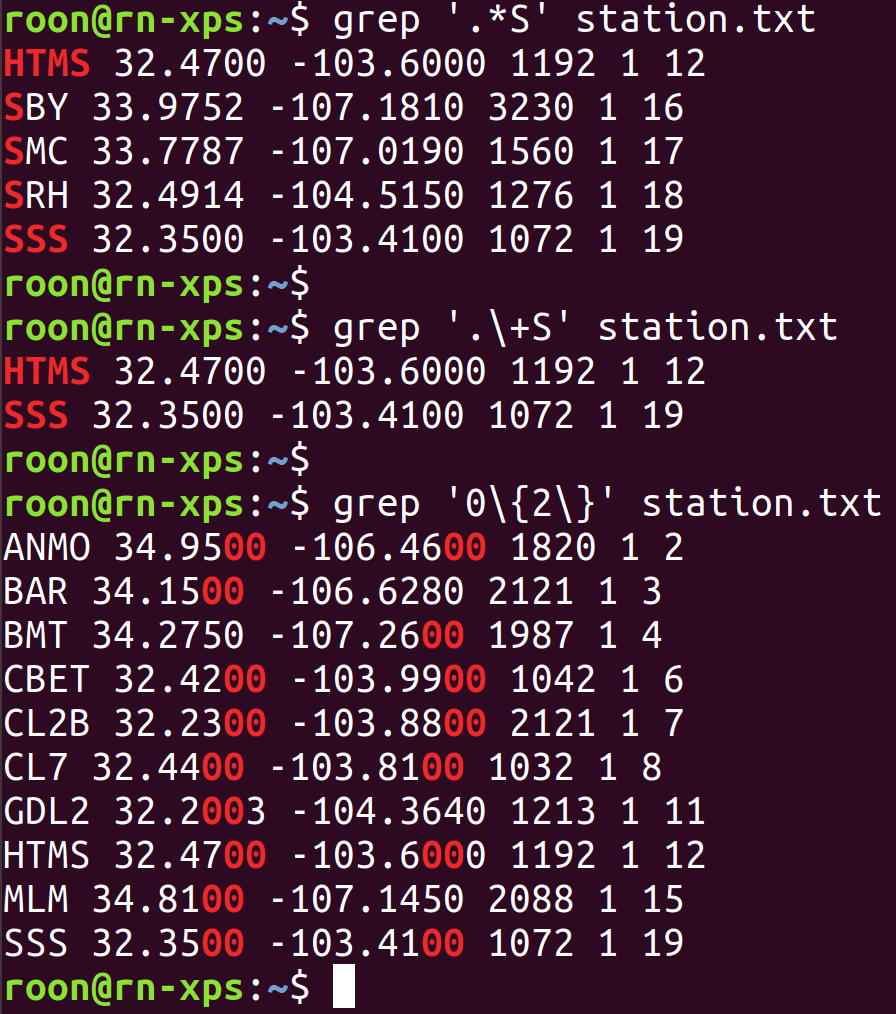
\includegraphics[width=.6\textwidth]{../figures/grep_examples2.png}	
	\end{center}
\end{frame}

\begin{frame}
	\frametitle{{\tt grep} Summary}
	\begin{center}
		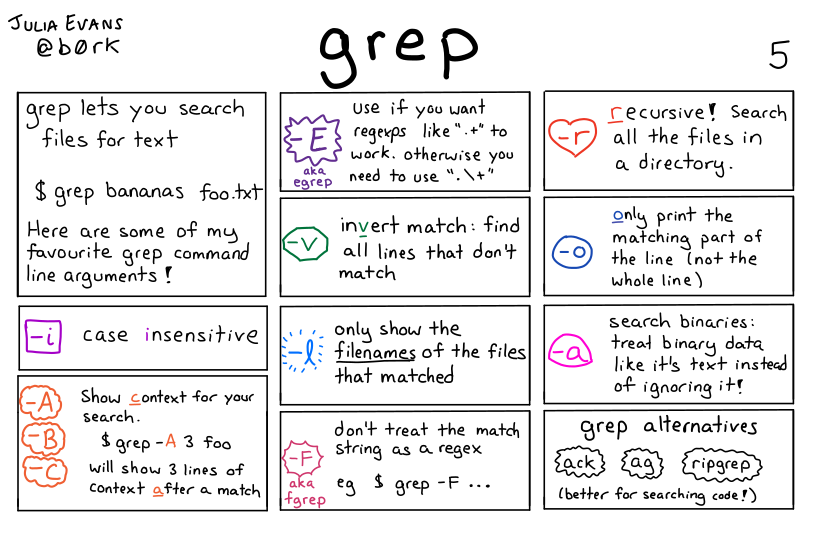
\includegraphics[width=\textwidth]{../figures/bork_grep.png}	
	\end{center}
	\begin{flushleft}
	\tiny{\emph{\url{https://wizardzines.com/comics/}}}
	\end{flushleft}	
\end{frame}

\begin{frame}
	\frametitle{{\tt sed} stream editor}
	\begin{itemize}
	\item Edit input line by line via command line 
	\item Most common use: find-and-replace on text files
	\end{itemize}

	\begin{center}
	{\tt sed 's/string1/string2/g' in\_file > out\_file}
	\end{center}

	\begin{itemize}
	\item Replace every occurrence of {\tt string1} in {\tt in\_file} with {\tt string2}, output is redirected to {\tt out\_file}
	\item {\tt s} in command string is for \emph{subsitute}
	\item {\tt g} means \emph{global} -- subsitute for every match, not just the first one
	\item {\tt sed -i} will change file in place ({\tt in\_file} would contain {\tt string2})
	\end{itemize}

\end{frame}

\begin{frame}
	\frametitle{{\tt sed} Example}
	\begin{center}
		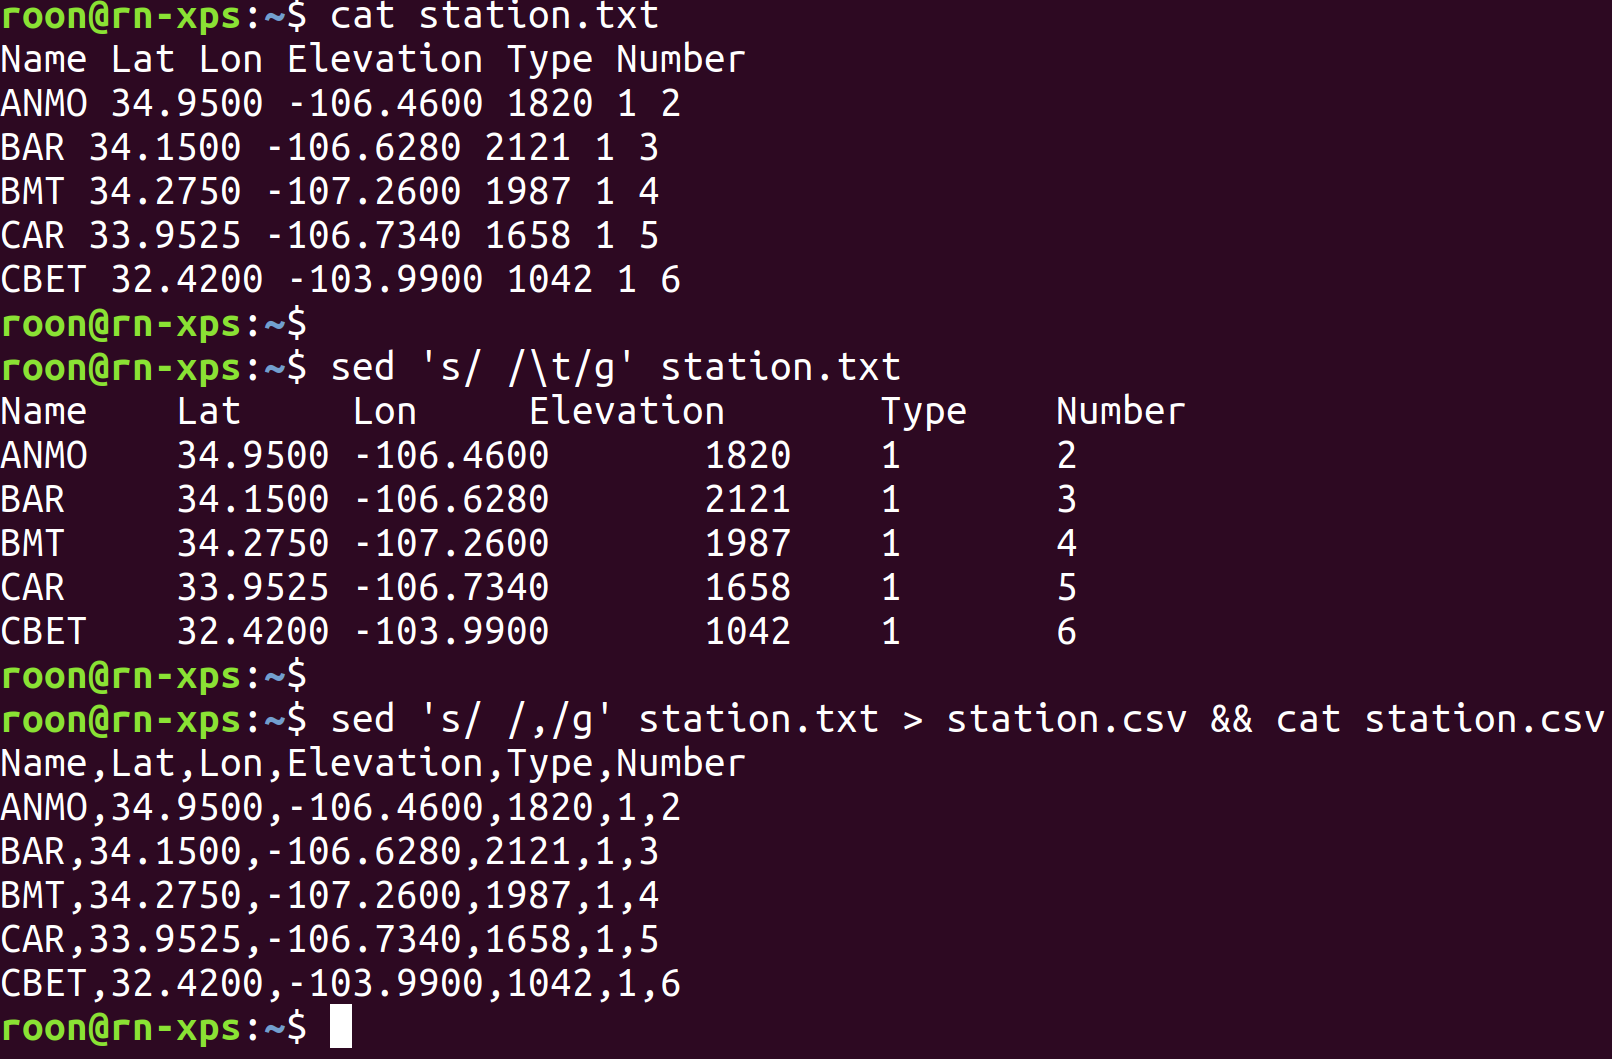
\includegraphics[width=\textwidth]{../figures/sed_example.png}	
	\end{center}
\end{frame}


\begin{frame}
	\frametitle{{\tt sed} Example}
	\begin{center}
		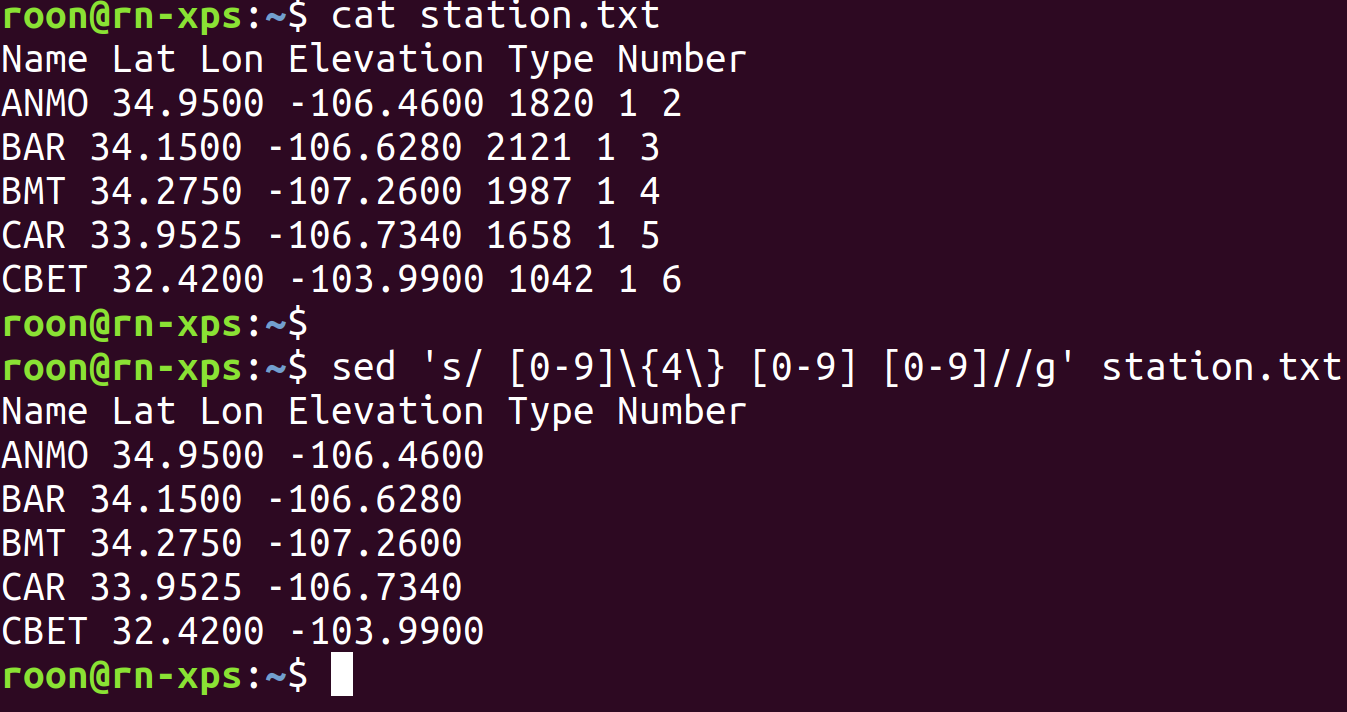
\includegraphics[width=\textwidth]{../figures/sed_example2.png}	
	\end{center}
\end{frame}


\begin{frame}
	\frametitle{{\tt sed} Summary}
	\begin{center}
		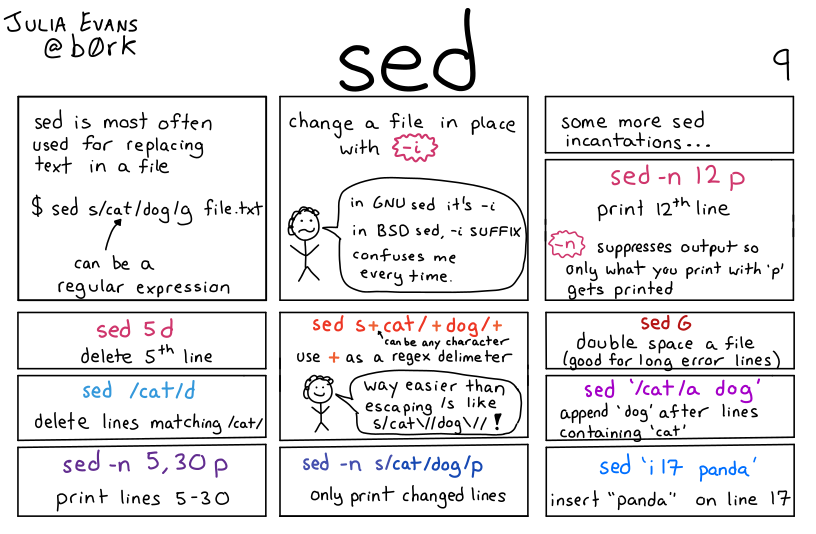
\includegraphics[width=\textwidth]{../figures/bork_sed.png}	
	\end{center}
	\begin{flushleft}
	\tiny{\emph{\url{https://wizardzines.com/comics/}}}
	\end{flushleft}	
\end{frame}


\begin{frame}
	\frametitle{{\tt awk}}
	\begin{itemize}
		\item Programming language to process files of text, reads input a line at a time
		\item Does floating point math
		\item Uses:
			\begin{itemize}
				\item Get the fourth, sixth, and 27th column of the file?
				\item Reorder columns
				\item Calculate the difference between numbers in 5th and 6th columns, divided by the square root of the sum of squares of the numbers inthe first 3 columns
				\item Get the all entries that are within a certain range of numbers (e.g., geographic bounding boxes)
				\item \dots
			\end{itemize}
	\end{itemize}
\end{frame}


\begin{frame}
	\frametitle{{\tt awk}}
	\begin{itemize}
		\item awk program is a sequence of {\tt pattern \{action\}} statements operating on a file
		\item If {\tt pattern} matches, {\tt action} is executed
		\item File treated as sequence of records (by default each line is a record)
		\item Each record is broken into a sequence of fields (columns), separated by FS (field separator), whitespace by default
		\item Each field is assigned to a variable: {\tt \$1} through {\tt \$NF} where {\tt NF} is a special variable for total number of fields; {\tt \$0} contains the complete line
	\end{itemize}
\end{frame}

\begin{frame}
	\frametitle{{\tt awk}}
	\begin{center}
		{\tt awk 'command string' files} 
	\end{center}

	\begin{itemize}
		\item {\tt command string} is of the form {\tt pattern \{action\}} and can have many pattern-action pairs
		\item Example: {\tt awk 'NF > 3 \{print \$4\}' some\_file.txt}
		\item If there are more than 3 fields, print out the 4th field.
	\end{itemize}
\end{frame}

\begin{frame}
	\frametitle{{\tt awk -F/-f/-v}}
	Change Field Separator:
	\begin{itemize}
		\item {\tt awk -F} option changes field separator
		\item To work on CSV files: {\tt awk -F, '\{\dots\}' somefile.csv}
	\end{itemize}

	Provide program in separate file
	\begin{itemize}
		\item {\tt awk -f awk-script somefile.txt} 
		\item instead of defining the program text on the command line, provide it in a separate file. 
	\end{itemize}

	Assign a value to a variable:
	\begin{itemize}
		\item {\tt awk -v var=value '\{\dots\}' somefile.txt} 
		\item assigns {\tt value} to program variable {\tt var}
		\item easy way to pass values from shell scripts into awk (e.g. lat-lon bounds)
		\item can use {\tt var} in script (no leading \$ just `{\tt var}' to reference) 
	\end{itemize}

\end{frame}

\begin{frame}
	\frametitle{{\tt awk} print (\& other functions)}
	\begin{itemize}
		\item {\tt print} is most common action
		\item awk implements range of string \& arithmetic functions, e.g.:
		\begin{itemize}
			\item {\tt substr(s,i,n)} return substring of string s, starting at index i, of length n (length can be 	ommitted)
			\item {\tt sqrt(x)} returns square root of x
			\item {\tt atan2(x,y)} returns arctan of y/x between $-\Pi$ and $\Pi$
			\item check man pages for more
		\end{itemize}
		\item you can write your own functions (with if and while and for)
		\item worth to read the documentation / manuals / books to dive deeper
	\end{itemize}
\end{frame}

\begin{frame}
	\frametitle{{\tt awk} Example}
	\begin{center}
		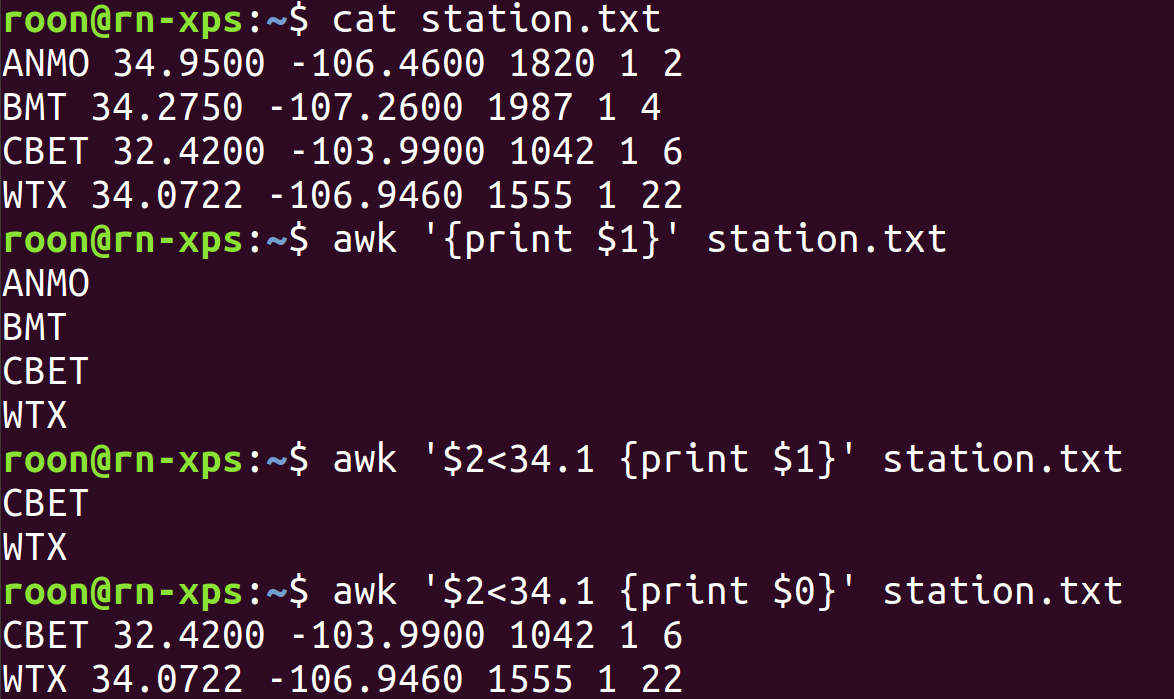
\includegraphics[width=\textwidth]{../figures/awk_examples.png}	
	\end{center}
\end{frame}

\begin{frame}
	\frametitle{{\tt awk} Example}
	\begin{center}
		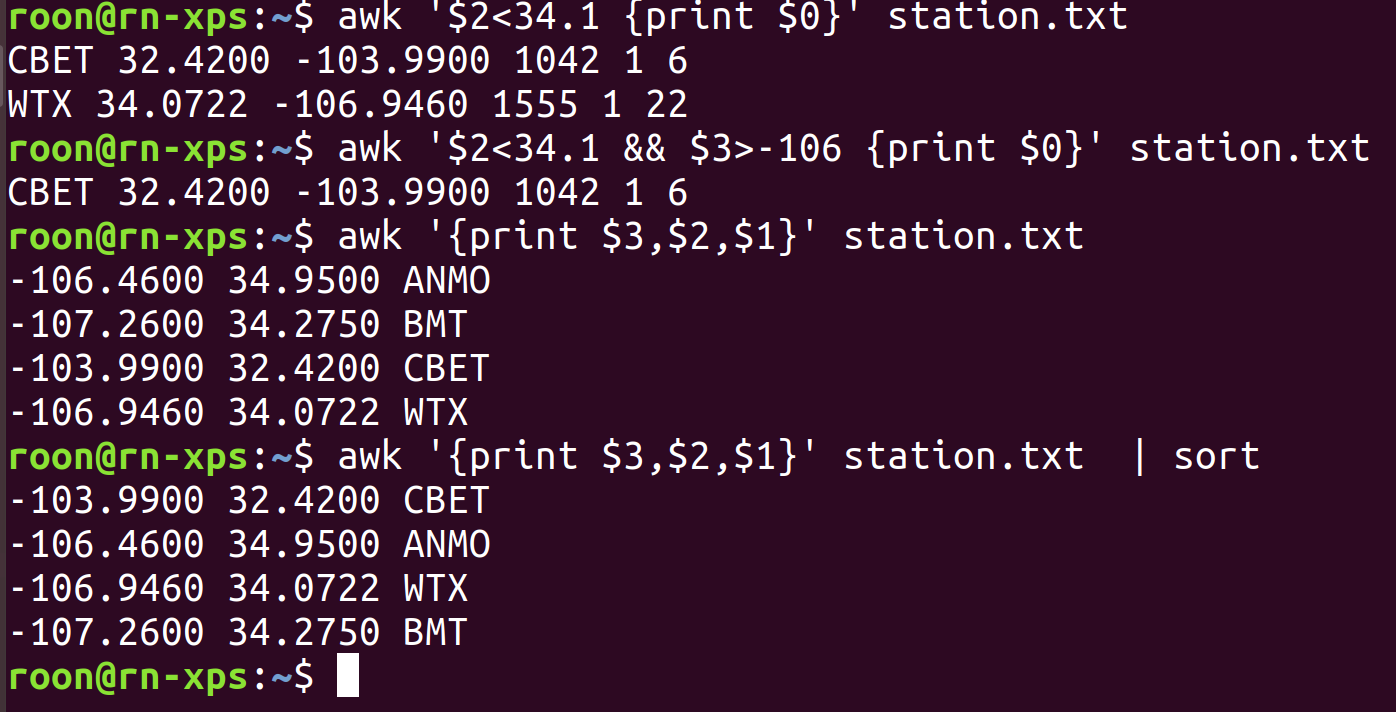
\includegraphics[width=\textwidth]{../figures/awk_examples2.png}	
	\end{center}
\end{frame}

\begin{frame}
	\frametitle{{\tt awk} Summary}
	\begin{center}
		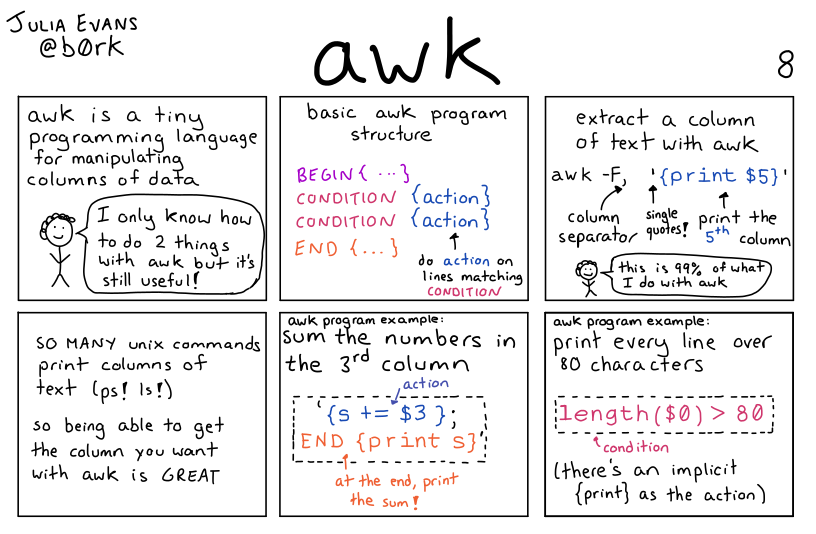
\includegraphics[width=\textwidth]{../figures/bork_awk.png}	
	\end{center}
	\begin{flushleft}
	\tiny{\emph{\url{https://wizardzines.com/comics/}}}
	\end{flushleft}	
\end{frame}

\end{document}
